\chapter{А на бумаге записать можно? Нотная грамота}
\label{ch:notes}

На определенном этапе своего развития человек может захотеть \emph{почитать} музыку, вместо того, чтобы её \emph{послушать}.

Нотную грамоту --- способ записи музыки на бумаге\footnote{Конечно, в наше время <<запись на бумаге>> звучит, гм, архаично. Зато понятно. Давйте договоримся, что когда употребляется <<бумага>>, подразумевается \emph{любой} способ отображения письма: бумага, экран монитора, проектор,\ldots}, нельзя назвать эталоном простоты. Как и любой другой язык, она формировалась долго: обрастала традициями, упрощалась, снова обрастала и т.д. Уважая гениальность предков, мы изучим её такой, какая она есть, и постораемся понять, почему она такая.

Начнём с основ:

\begin{Definition}[Нота]
    \emph{Нота} --- это \emph{буква} музыкального письма, позволяющая определить \emph{высоту} (частоту колебаний) и \emph{длительность} музыкального звука. 
\end{Definition}


\section{А словами как назвать? Названия нот}
\label{ch:notes:names}

В Русской традиции принято использовать следующие семь \emph{названий} нот, которые приведены в порядке возрастания высоты звука (частоты колебаний основного тона): 
\begin{center}
    ДО, РЕ, МИ, ФА, СОЛЬ, ЛЯ, СИ.
\end{center}

Такие названия нот удобны тем, что их можно \emph{петь}: тянуть последнюю гласную пока воздуха хватает. Самый совершенный музыкальный инструмент у человека всегда с собой --- его голос. Друзья, поверьте, есть такие люди, которые могут \emph{петь по нотам}! Их мало на нашей эстраде, но они есть. Только не надо думать, что если вы споёте, например, <<ДО-О-О-О>>, то сам собой прозвучит звук нужной высоты. Не льстите себе! Такое может сделать только мастер. Он любую гласную вытянет в \emph{унисон} с любым сыгранным не гитаре звуком.

Приведенные \emph{названия} нот определяют музыкальный звук внутри октавы\footnote{Об октавах и полутонах см. раздел \ref{ch:music:tone}}. Мы уже знаем, что в октаве содержится 12 музыкальных звуков. Так вот принято считать, что октава начинается с ноты ДО. Отсчитав от ДО 12 полутонов вверх/вниз, попадем на ноту ДО следующей/предыдущей октавы. Таким образом весь диапазон музыкальных звуков разбит на октавы, начинающиеся с ноты ДО. Видно, что из 12 звуков октавы только 7 получили собственные названия, их положение внутри октавы приведено на рисунке \ref{fig:notes:names:main:RU}.

\begin{figure}[!ht]
    \centering
    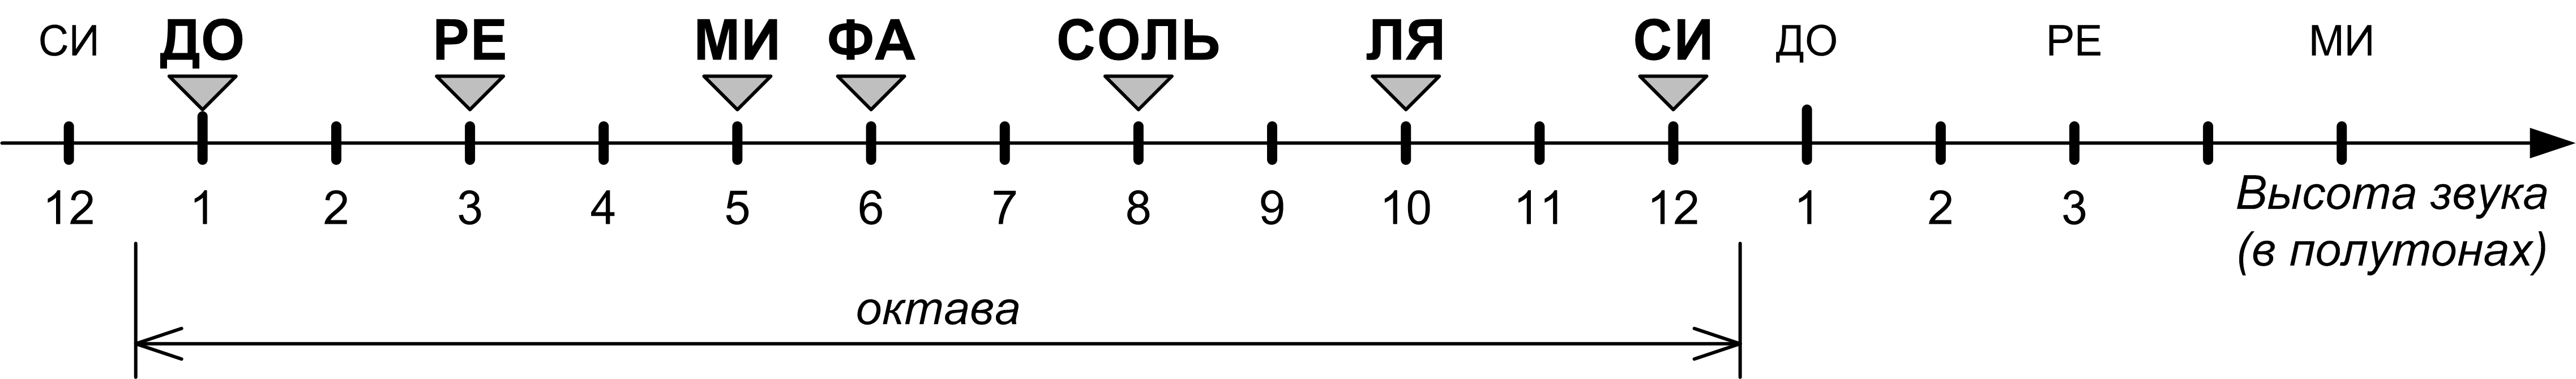
\includegraphics[width=\textwidth]{fig/notes/notes-main-ru} 
    \caption{Названия основных нот октавы RU}\label{fig:notes:names:main:RU}
\end{figure} 

Оставшиеся (12-7)=5 звуков не удостоились отдельных имен. Их имена формируются добавлением суффиксов <<-диез>> или <<-бемоль>> к стоящей по соседству (слева или справа) основной ноте. <<Диез>> повышает звук на полутон, а <<бемоль>> --- понижает. Итак между следующими основными нотами находится <<промежуточный>> звук (см. рисунок \ref{fig:notes:names:all:RU}).
\begin{enumerate}
    \item ДО и РЕ (этот звук может быть назван либо ДО-диез, либо РЕ-бемоль);
    \item РЕ и МИ (РЕ-диез или МИ-бемоль);
    \item ФА и СОЛЬ (ФА-диез или СОЛЬ-бемоль);
    \item СОЛЬ и ЛЯ (СОЛЬ-диез или ЛЯ-бемоль);
    \item ЛЯ и СИ (ЛЯ-диез или СИ-бемоль).
\end{enumerate}

\begin{figure}[!ht]
    \centering
    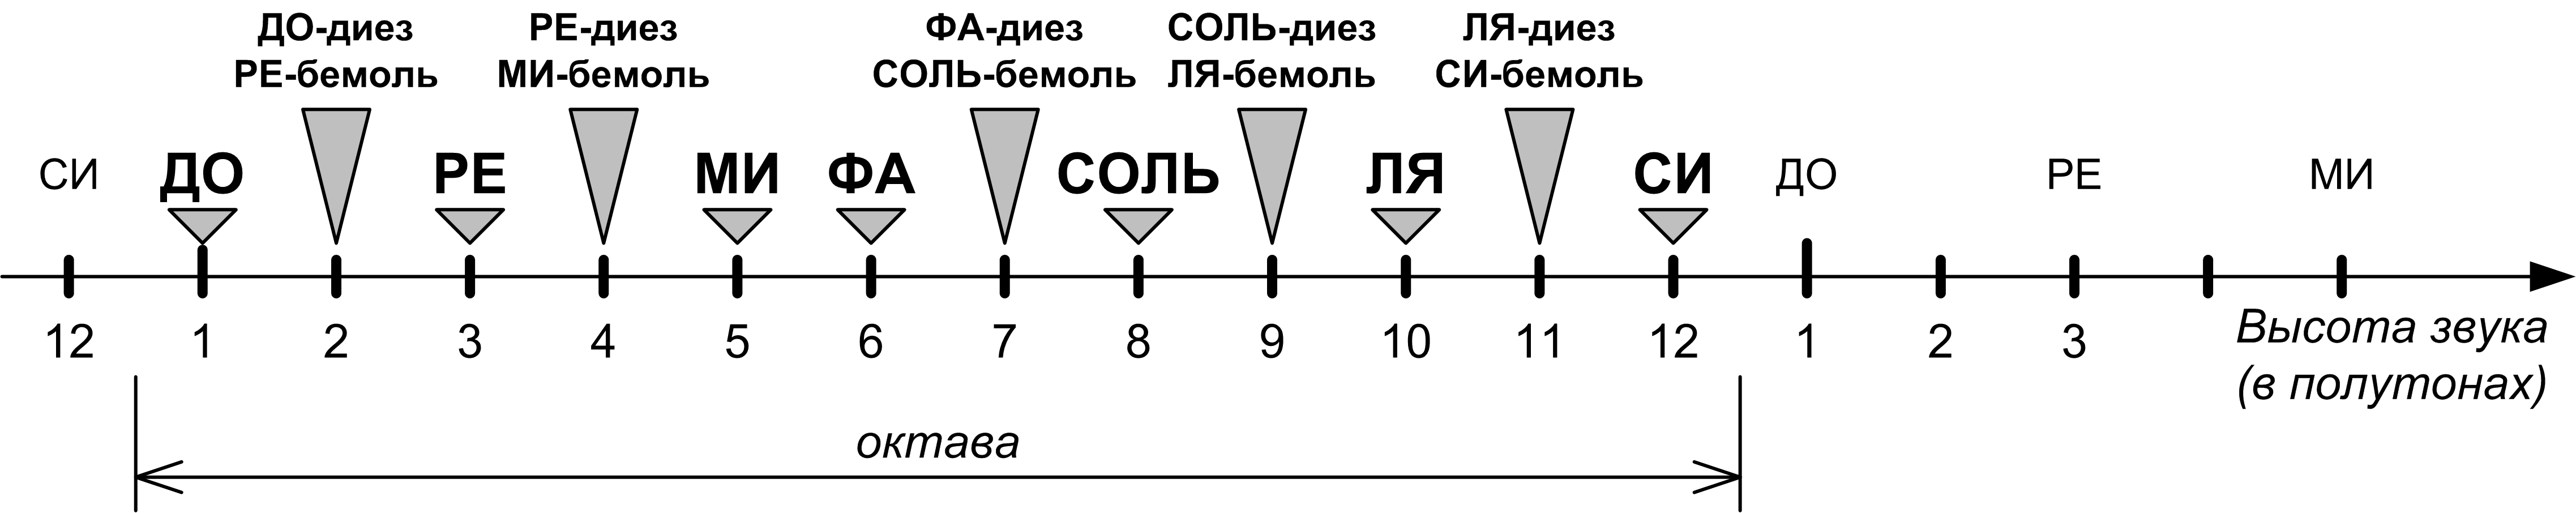
\includegraphics[width=\textwidth]{fig/notes/notes-all-ru} 
    \caption{Названия всех нот октавы RU}\label{fig:notes:names:all:RU}
\end{figure} 

Как видно, <<промежуточные>> ноты могут называться двояко. Какое из имен выбрать? Постараюсь ответить кратко: если вы читаете этот текст и узнаёте для себя что-то новое, то вам позволительно использовать любое\footnote{Это как грамотность в Русском языке: надеть или одеть? Одеть Надежду, надеть одежду! Чужак не осилит. Так что называйте как хотите, знающие друзья поправят, если что. Только помалкивайте на какой-нибудь музыкальной конференции в кругу маститых классических исполнителей}. Все 12 звуков октавы в порядке увеличения высоты:
\begin{center}
    ДО, ДО-диез, РЕ, РЕ-диез, МИ, ФА, ФА-диез, СОЛЬ, СОЛЬ-диез, ЛЯ, ЛЯ-диез, СИ
\end{center}

Когда октаву читают в нисходящем порядке, то грамотно использовать <<-бемоль>>:
\begin{center}
    СИ, СИ-бемоль, ЛЯ, ЛЯ-бемоль, СОЛЬ, СОЛЬ-бемоль, ФА, МИ, МИ-бемоль, РЕ, РЕ-бемоль, ДО
\end{center}

Отметим, что между МИ и ФА, а также между СИ и ДО, промежуточных звуков нет\footnote{Вам уже давно хочется сказать: <<Диез-бемоль! Какого чёрта? Почему? Зачем эти сложности?>> Друзья мои, болею за вас! Творится полный беспредел с точки зрения кодирования! Можно проще, но все привыкли. Знаете, это традиция, в которой есть смысл! Наберитесь терпения}: расстояние между ними --- один полутон. Однако никто не мешает, например, назвать ноту ДО как СИ-диез, или ноту МИ как ФА-бемоль. В устной речи так, конечно, никто не сделает, а вот при записи знаков нот на бумаге такое вполне допустимо, чтобы значки не <<наезжали>> друг на друга.

Американцы и англичане обозначают ноты буквами алфавита (см. также рисунок \ref{fig:notes:names:all:EN}):
\begin{center}
    A(ля), B(си), C(до), D(ре), E(ми), F(фа), G(соль).
\end{center}

\begin{figure}[!ht]
    \centering
    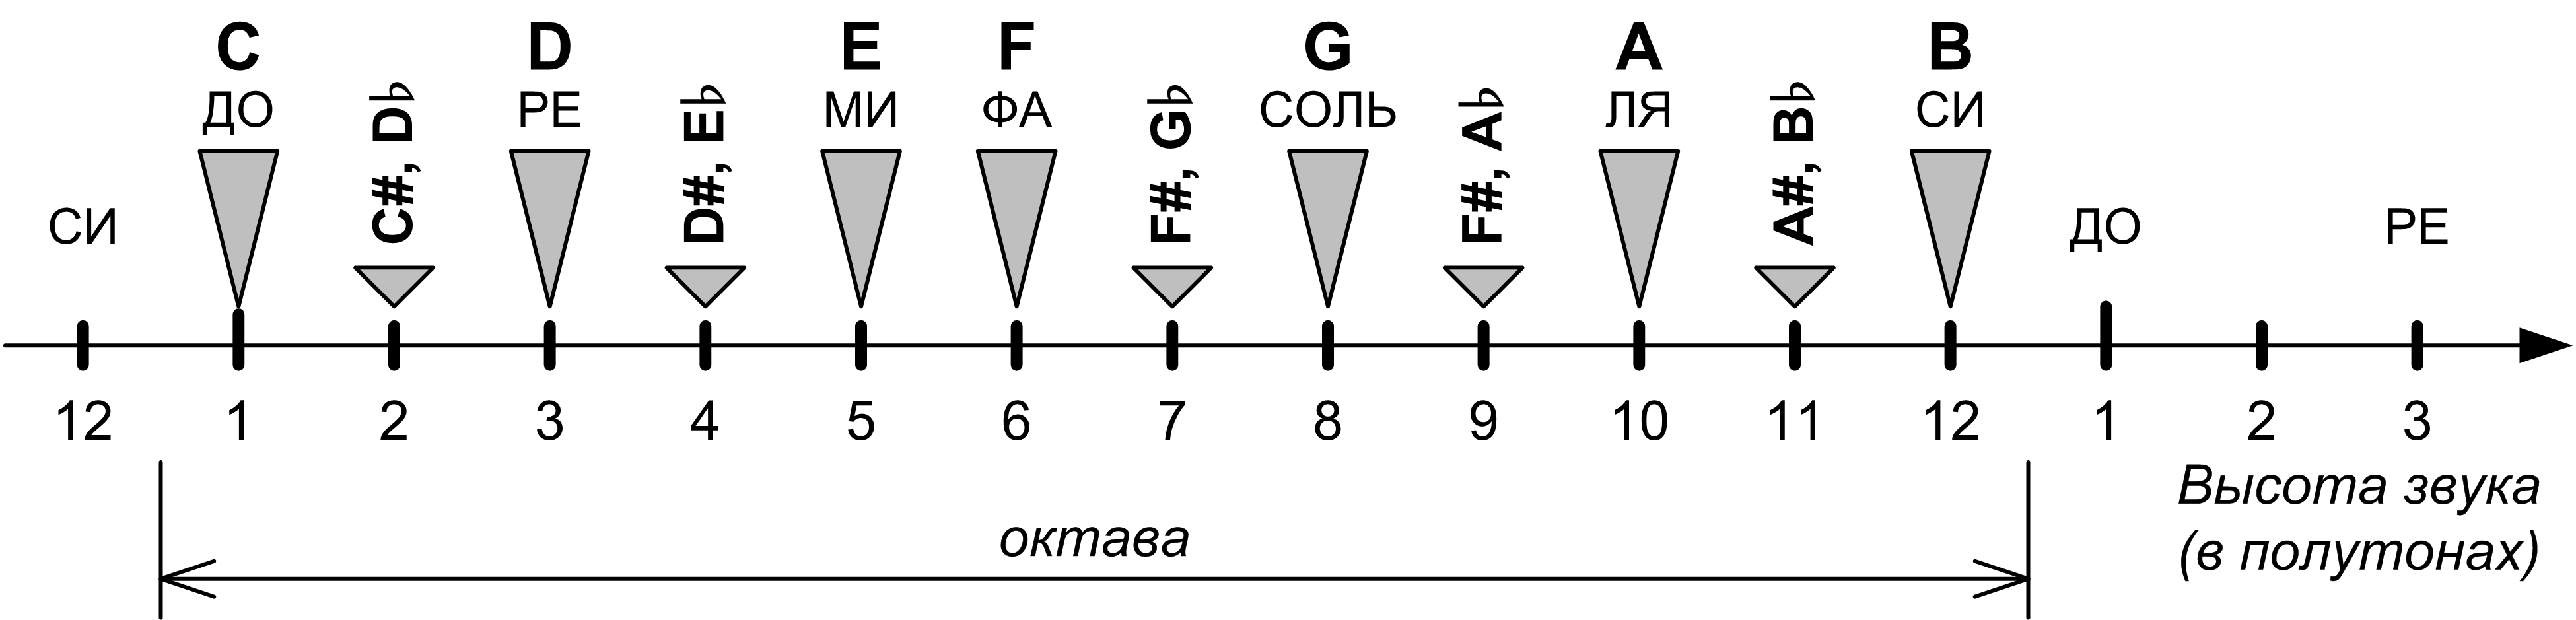
\includegraphics[width=\textwidth]{fig/notes/notes-all-en} 
    \caption{Названия всех нот октавы EN}\label{fig:notes:names:all:EN}
\end{figure} 

Важно запомнить эти обозначения прямо сейчас! Они слишком часто используются в гитарной музыке. Причем вместо суффикса <<-диез>> изпользуется значок $\sharp$, а вместо <<-бемоль>> --- $\flat$. Например, нота ДО-диез может быть обозначена как $C\sharp$ или как $D\flat$.

Знаки $\sharp$ и $\flat$ часто заменяют на окончания <<is>> и <<es>> соответственно. Особенно в компьютерных текстах, так как, прямой ввод с клавиатуры этих символов обычно затруднён. То есть, если вы получили электронное письмо от музыканта и встретили в нём, например, странное слово <<fis>>, не пугайтесь --- это всего лишь $F\sharp$ (ФА-диез). Встретился <<bes>>? --- это $B\flat$ (СИ-бемоль).

\begin{Example}[Страшная сказка об английских обозначениях нот]
    И жили они, не тужили с октавой, начинающейся с ЛЯ, то есть, как и положено, c A\ldots Ага, вроде всё логично и просто, как азбука. Английский алфавит читается: A-эй, B-би, C-си, D-ди, E-и, F-эф, G-джи, H-эйч,\ldots Как вдруг, в результате спонтанного шизоидного сдвига, всем вдруг стало ясно, что октава должна начинаться с ДО. Причина сего интересна не только психиатрам! Если вы разберетесь с \emph{музыкальным ладом}, то вы сами дадите этому заскоку рациональное объяснение. И порядок немного сломался, ибо стало: CDEFGAB. А потом кому-то показалось, что для ноты СИ буквы не хватило! И назначили для ноты СИ очередную свободную латинскую букву H! Гитаристам с латиницей дело иметь придется часто, поэтому запомните приведенное соответствие и будьте готовы к тому, что для обозначения ноты СИ может быть использована латинская буква H. Все даже чуть сложнее\ldots Если вы увидели книжку, где используется <<H>>, то знайте, что это <<СИ>>. Но не падайте духом, если вдруг увидите, что там же используется и латинская <<B>>! В данном клиническом случае <<B>> будет обозначать ноту <<CИ-бемоль>>! Боже, короче говоря, упаси от такого!
\end{Example}

Напоследок осталось отметить, что для того, чтобы назвать \emph{музыкальный звук}, нужно определить не только ноту но и октаву, к которой он относится. Так как названия нот в пределах октавы повторяются, то октавную систему удобно представлять себе в виде спирали, как на рисунке \ref{fig:notes:names:octave}.

\begin{figure}[!ht]
    \centering
    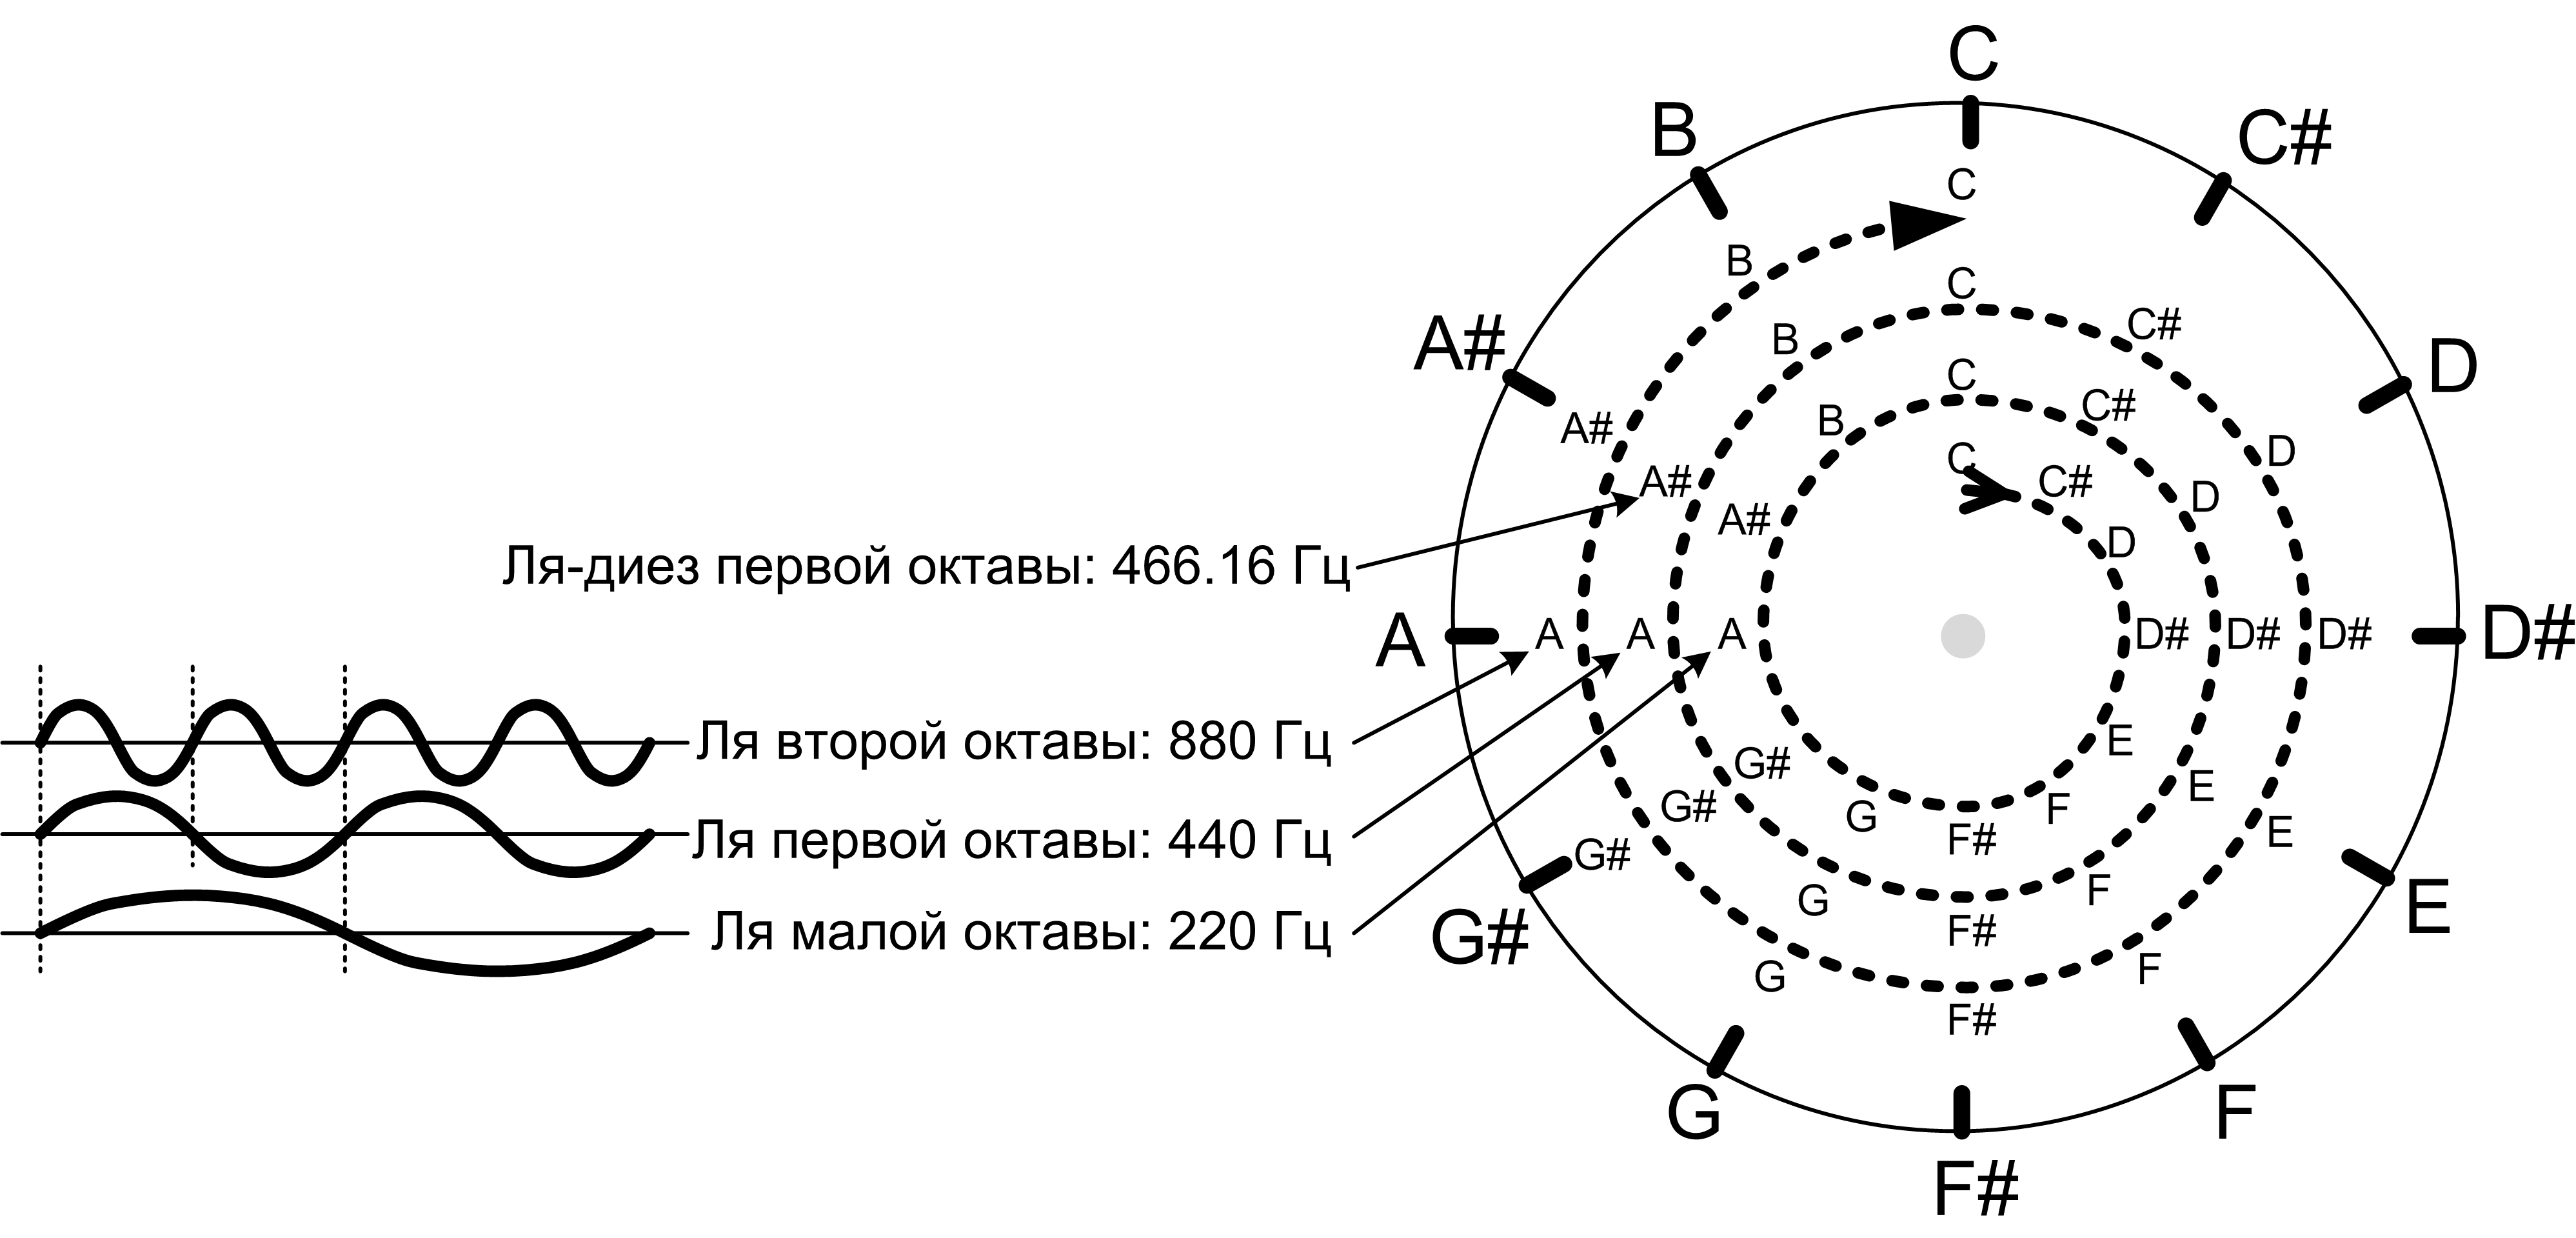
\includegraphics{fig/intervals/octave-spiral} 
    \caption{Пооктавная цикличность музыкальных звуков}\label{fig:notes:names:octave}
\end{figure} 

Названия использующихся в музыке октав приведены в таблице \ref{tab:notes:names:octaves}. Также в таблице приведена частота основного тона входящей в октаву ноты ЛЯ. Частоты остальных нот при желании можно вычислить по формуле \eqref{eq:music:tone:frequency}, надо лишь полутона правильно посчитать. Отдельно \emph{выделены} те октавы, которые входят в диапазон шестиструнной гитары. Справедливости ради следует сказать, что её диапазон звучания полностью включает лишь малую и первую октавы.

\begin{table}[!ht]
    \centering
    \caption{Октавы}
    \label{tab:notes:names:octaves}
    \begin{tabular}{ll}
        \hline\hline
        Название октавы         & Частота ноты Ля, Гц \\
        \hline\hline
        
        Субконтроктава          & 27.5 \\
        Контроктава             & 55   \\
        \emph{Большая октава}   & 110  \\
        \emph{Малая октава}     & 220  \\
        \emph{Первая октава}    & A4=\fbox{440}  \\
        \emph{Вторая октава}    & 880  \\
        Третья октава           & 1760 \\
        Четвертая октава        & 3520 \\
        Пятая октава            & 7040 \\
        \hline
    \end{tabular}
\end{table}

Все же стоит дать краткий ответ на вопрос: <<почему не все 12 нот октавы получили индивидуальные имена?>>. Дело в том, что из <<основных>> семи нот можно составить гармоничную мелодию, а оставшиеся <<промежуточные>> ноты при этом будут использоваться крайне редко --- так зачем им имена? За подробным ответом пожалуйте в царство гармонии, в раздел \ref{ch:harmony}.


\section{Что тут зашифровано? Запись нот}

Чтобы пронести музыку сквозь время, её нужно уметь записать на бумаге. И само собой, нужно уметь прочитать записанное, чтобы молчаливые ноты наконец <<заговорили>> с помощью музыкального инструмента.

Музыкальный диапазон гитары невелик, поэтому нотная запись для нее даже проще, чем для более <<матёрых>> инструментов, таких как, например, фортепиано. Гитаристы чаще всего столкнутся с чем-то подобным:

\begin{center}    
    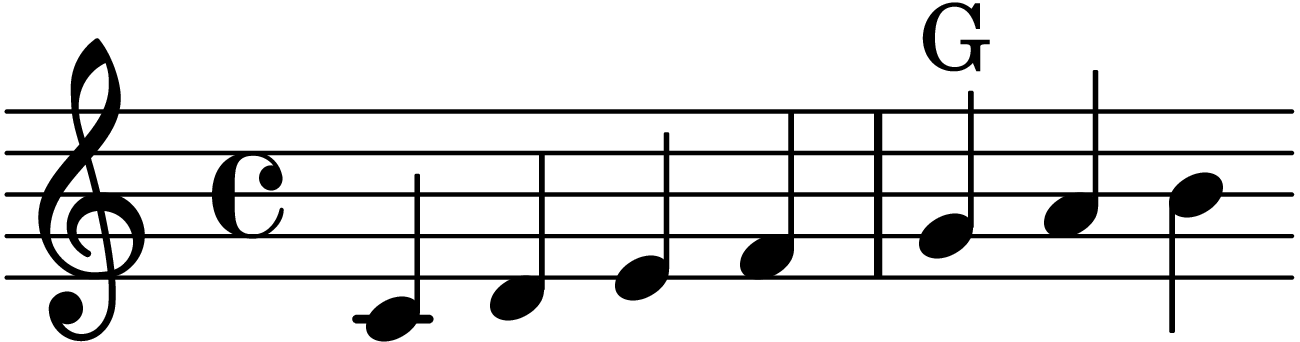
\includegraphics{fig/notes/octave-little}
\end{center}    

Разберемся с тем, что мы видим на рисунке:
\begin{itemize}
    \item Одну линейку \emph{нотоносца} --- пять параллельных горизонтальных линий, на которых размещаются нотные знаки. Собственно ноты, определяющие высоту и длительность музыкального звука, будут писаться либо на линии, либо в промежутке между соседними линиями.
    
    \item Первый нотный знак на нотоносце --- \emph{скрипичный ключ}. Своим финальным завитком он обвивает вторую снизу линию нотоносца, на которой будут записываться все ноты СОЛЬ (G) \emph{малой} октавы\footnote{Для других музыкальных инструментов, в первую очередь, для фортепиано, скрипичный ключ показывает положение СОЛЬ \emph{первой} октавы. Вообще-то ноты для фортепиано пишутся на двух линейках нотоносца, причем на одной линейке ноты пишут в скрипичном ключе, а на второй --- в \emph{басовом}. Для гитары же, музыкальный диапазон которой легко укладывается в три с копеечкой октавы, используют всего одну линейку нотоносца и ноты пишут в скрипичном ключе, но октавой ниже. То есть для фортепиано, нота записанная на второй линейке --- это СОЛЬ первой октавы, а для гитары это будет СОЛЬ, но октавой ниже: СОЛЬ малой октавы}. Скрипичный ключ --- один из нескольких <<ключевых>> знаков, которые определяют какой высоты музыкальные звуки будут писаться на той или иной линиии нотоносца. Вся гитарная музыка пишется на одной линейке нотоносца под скрипичным ключом.
    
    \item Второй знак на нотоносце после скрипичного ключа --- латинская буква <<C>>. Этот знак определяет \emph{музыкальный размер} <<четыре четверти>>. Вместо буквы <<C>> может быть написана дробь:
    
    \[\frac{4}{4}\]
        
    Размеры могут быть самыми разными, но <<четыре четверти>> --- один из самых популярных и удостоился более простого обозначения: <<C>>.
    
    Итак, после знака ключа (в гитарном случае всегда скрипичного), определяющего положение нот по высоте, следует знак, определяющий размер или, что то же, длительность \emph{такта}. Мы уже разбирались, что музыка пульсирует периодически повторяющимися во времени акцентами (см. раздел \ref{ch:music:volume}). Так вот \emph{такт} --- это и есть этот период времени, только измеренный в долях условной музыкальной <<единицы>> длительности. А этой самой условной единице в свою очередь может быть сопоставлен абсолютно любой интервал времени, так как одну и ту же музыку можно сыграть как медленно, так и быстро. 
    
    На нотоносце такты отделяются друг от друга вертикальной чертой, для удобства такты иногда нумеруются. В нашем случае такт длится четыре четверти условной единицы времени, то есть как раз эту самую единицу времени. Обратите внимание, что первая вертикальная черта появляется после четвертой ноты. Надо ли говорить, что все эти ноты --- четвертные?
    
    Обычно автор музыкального произведения заранее оговаривает, как быстро его играть, задавая, например, длительность <<целой>> или <<четвертной>> ноты в долях минуты. Это уже называется \emph{темпом}. Например, если автор говорит, что четвертную ноту играют в темпе 120, то это значит, что четвертная нота будет длиться одну стодвадцатую долю минуты или половину секунды.
    
    \item Третий знак на приведенном выше рисунке похож на 6 следующих за ним. Это и есть ноты, определяющие высоту и длительность музыкальных звуков. Нота изображается маленьким овалом, распологающимся на линии нотоносца или между соседними линиями. Положение ноты на линиях нотоносца определяет высоту музыкального звука, а особенности её изображения (закрашенность, наличие <<хвостиков>>) --- длительность. Длительность ноты измеряется в долях уже упоминавшейся условной <<единицы>> длительности.
    
    В нашем случае первая нота --- это нота ДО (C) малой октавы длительностью в одну четверть. Как можно видеть, она находится на первой <<добавочной>> линии нотоносца. Добавочные линии могут появляться как снизу, так и сверху нотной линейки. На рисунке представлена последовательность из 7 нот малой октавы: ДО, РЕ, МИ, ФА, СОЛЬ, ЛЯ, СИ.
    
    Чем ниже находится нота на нотной линейке, тем ниже музыкальный звук, ей соответствующий. Особенности изображения нот обсудим чуть позже.
        
    Обратите внимание, что нота СОЛЬ (подписана <<G>> над соотвествующей нотой) находится на второй линии нотоносца, на которую так явно указывает скрипичный ключ.
    
    Без добавочных знаков на нотоносце изображаются только ДО, РЕ, МИ, ФА, СОЛЬ, ЛЯ, СИ. Причем все просто: если нота располагается на линии, то следующая за ней располагается в промежутке, следующая снова на линии и т.д.
\end{itemize}

Самая низкая нота стандартно настроенной гитары --- нота МИ большой октавы. Пять нот от МИ до СИ большой октавы:
\begin{center}    
    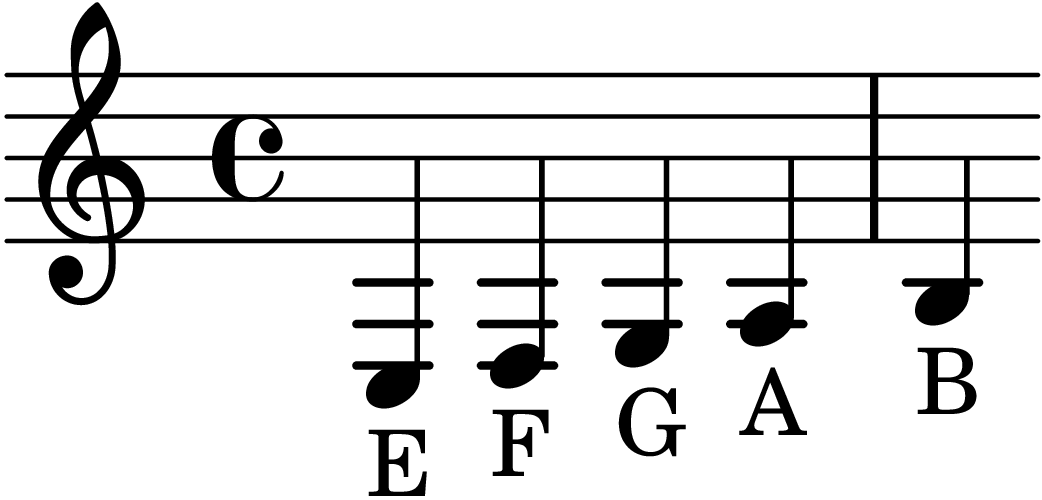
\includegraphics{fig/notes/octave-big}
\end{center}

Семь нот от ДО до СИ первой октавы:
\begin{center}    
    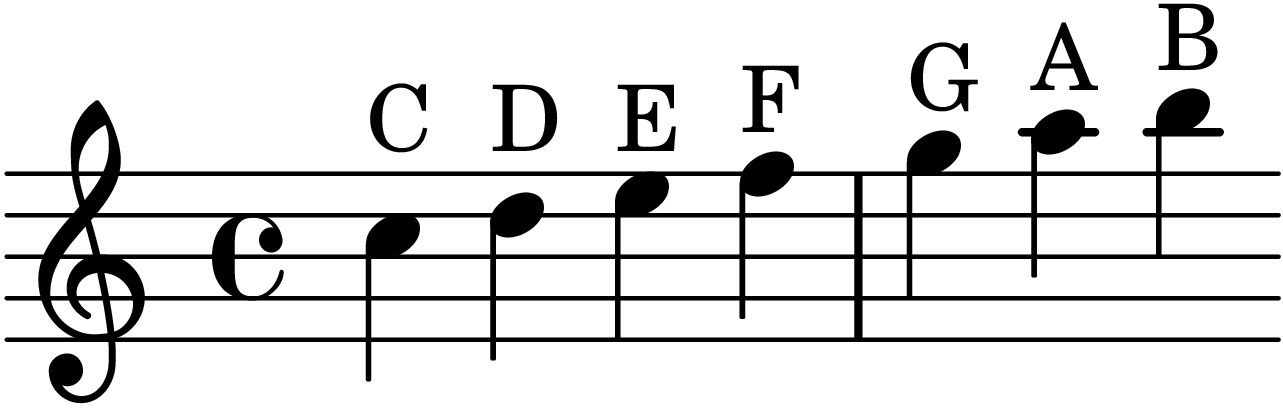
\includegraphics{fig/notes/octave-first}
\end{center}

И остается еще немного нот <<вверх>>, чтобы <<закрыть>> диапазон гитары (cемь нот ДО--СИ второй октавы):
\begin{center}    
    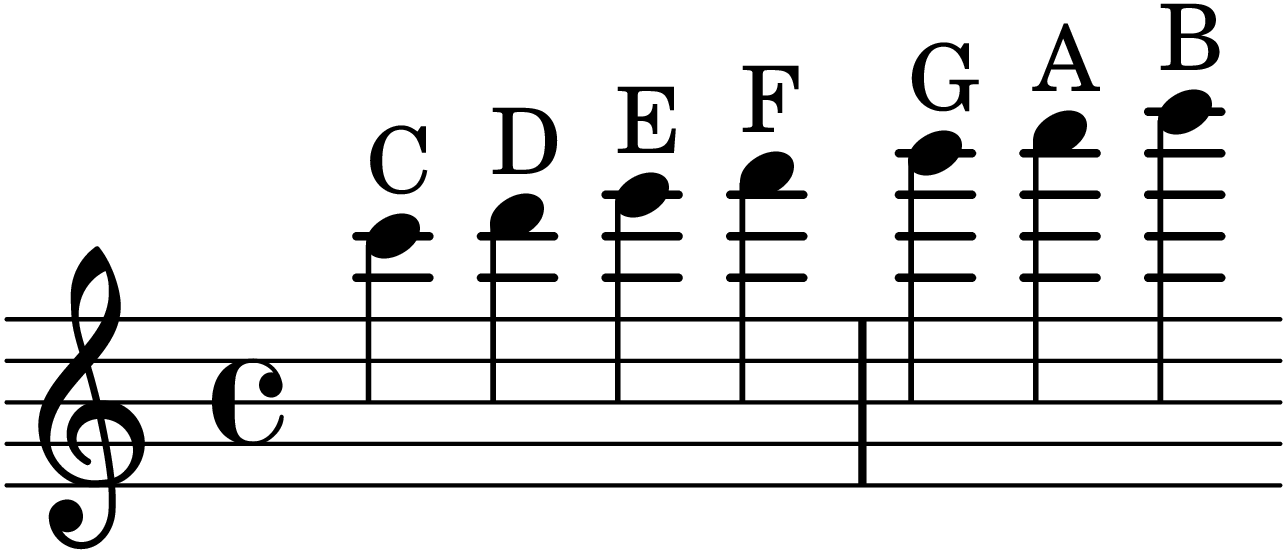
\includegraphics{fig/notes/octave-second}
\end{center}

Как определять высоту звука мы разобрались, теперь разберемся с длительностями:
\begin{center}    
    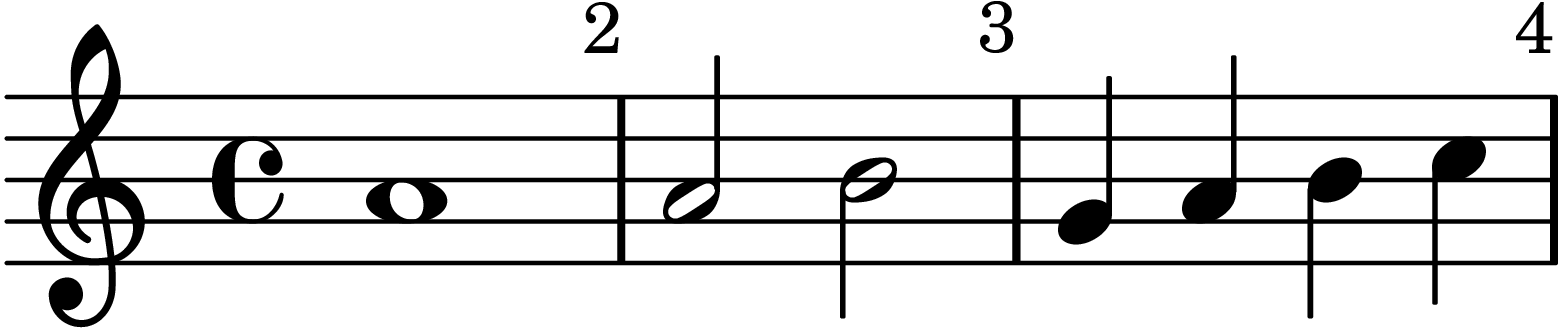
\includegraphics{fig/notes/time-4-4}
\end{center}

Музыканты должны неплохо знать рациональные дроби. Итак, мы знаем, что такт в данном случае длится одну условную единицу времени.
\begin{itemize}
    \item В первом такте (после знаков скрипичного ключа и размера <<C>>) изображена \emph{целая} нота ЛЯ малой октавы. Изображается она простым назакрашенным овалом. Такая нота звучит одну условную единицу времени. 
    
    \item Во втором такте звучат две \emph{половинные} ноты: ЛЯ и СИ. Изображается половинная нота незакрашенным овалом с <<прямым хвостиком>>, причем хвостик может быть направлен как вверх, так и вниз (чтобы смотрелось гармоничнее). Каждая из них звучит половину условной единицы, а вместе они заполнят такт.
    
    \item В третьем такте звучат четыре \emph{четвертные} ноты: СОЛЬ, ЛЯ, СИ, ДО. Овал закрашен, имеется прямой хвостик.
\end{itemize}

Заметили, как изменяется длительность нот: целая, половинная, четвертная\ldots Верно, дальше будут восьмые, шестнадцатые, тридцать вторые\footnote{Если кто-то из программистов или математиков дочитал до этих строк, приветствую! Да, это ничто иное, как двоичная система счисления} и т.д.

Возьмем такт, длящийся четверть условной единицы (размер $\frac{1}{4}$ после ключа) и проиллюстрируем: 
\begin{center}    
    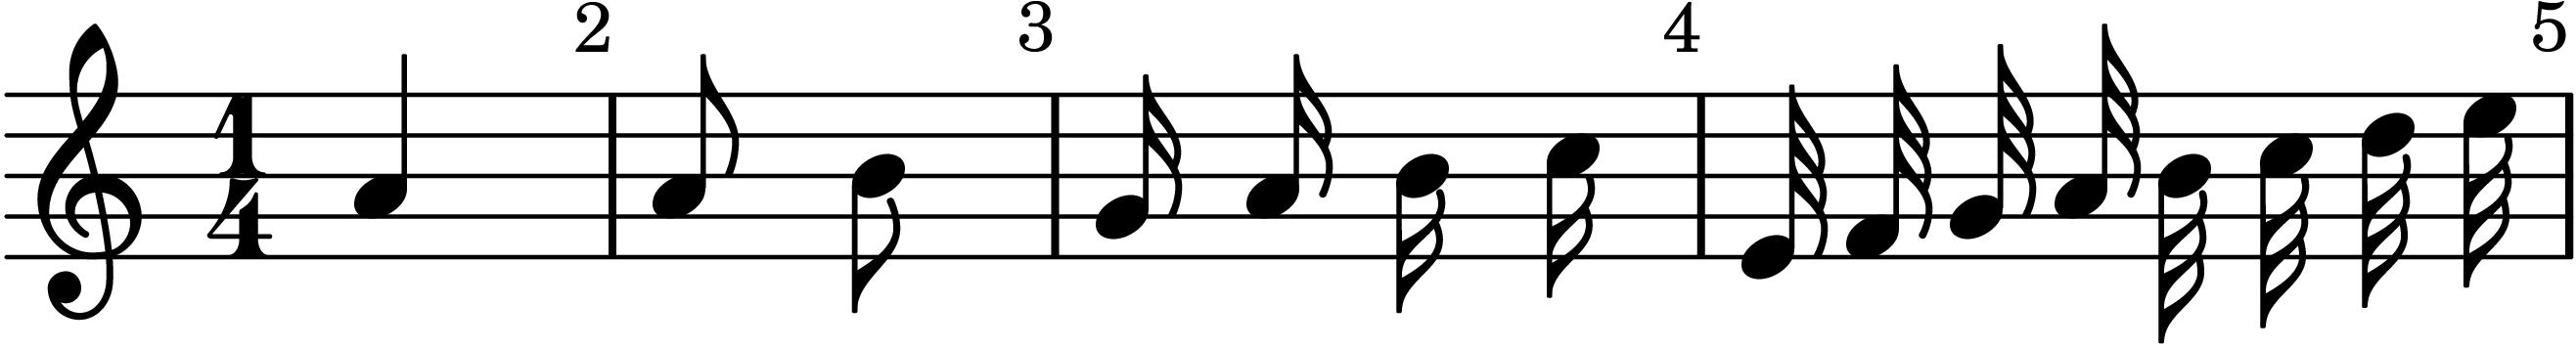
\includegraphics{fig/notes/time-1-4-beam-off}
\end{center}

\begin{itemize}
    \item Восьмые ноты (во втором такте) --- закрашенный овал и хвостик с одной засечкой (флажком). Восьмая нота длится одну восьмую условной единицы времени. Две восьмые ноты длятся $\frac{1}{8} + \frac{1}{8} = \frac{1}{4}$ часть условной единицы, то есть как раз заполняют <<четвертной>> такт.
    \item Шестнадцатые (в третьем такте) --- две засечки на хвостике.
    \item Тридцать вторые (в четвертом такте) --- три засечки.
\end{itemize}

Когда несколько нот одной длительности следуют друг за другом, чтобы не рисовать у каждой ноты засечки используют прямые линии --- ребра (вязки). Следующий фрагмент полностью идентичен предыдущему:
\begin{center}    
    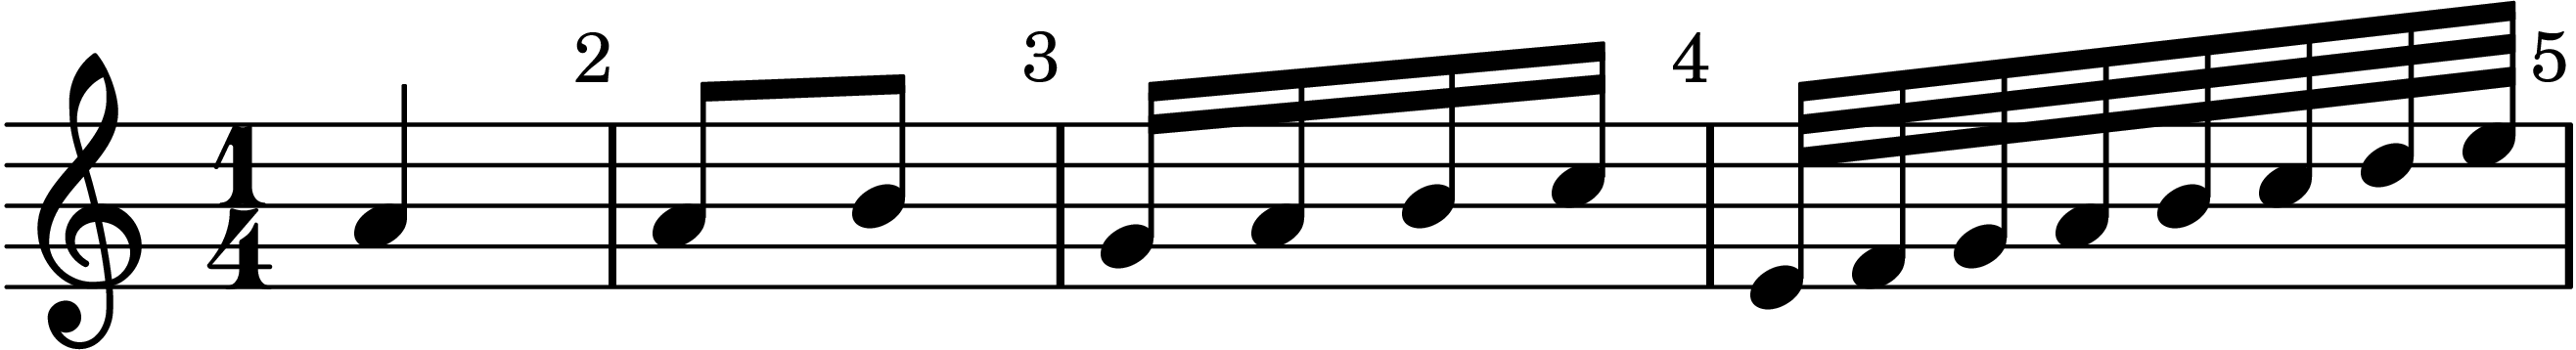
\includegraphics{fig/notes/time-1-4-beam-on}
\end{center}

Когда нужно <<создать>> ноту нестандартной длительности, используют значок \emph{лиги} (дуги), объединяющий две отдельно написанные ноты в одну:
\begin{center}    
    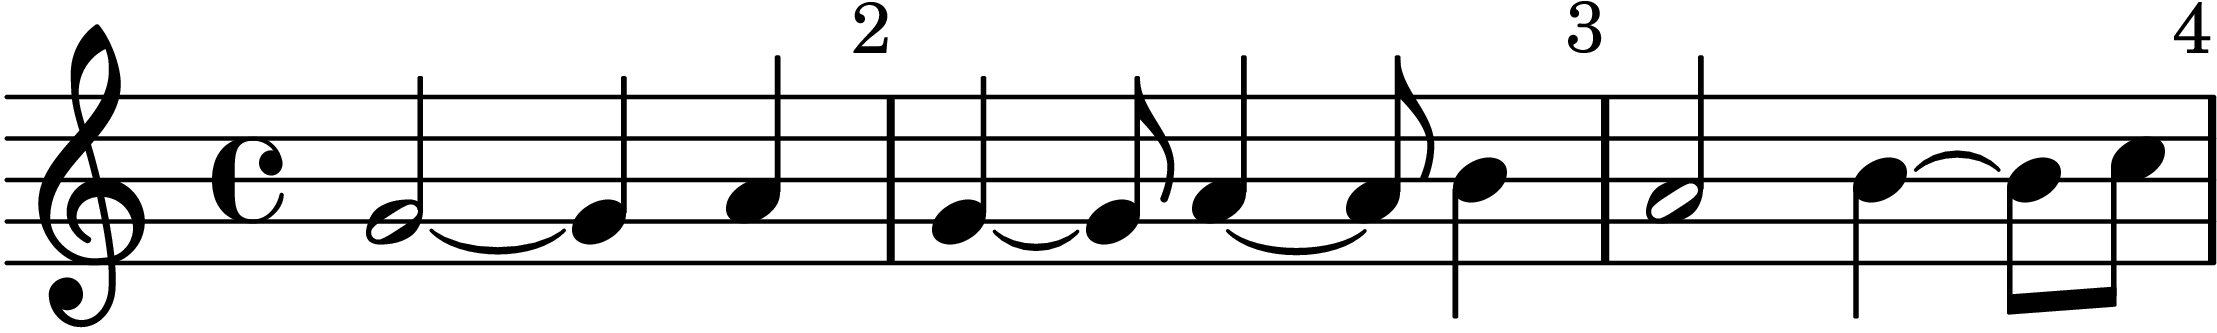
\includegraphics{fig/notes/tie}
\end{center}

\begin{itemize}
    \item В первом такте звучит две ноты СОЛЬ и ЛЯ: $\frac{3}{4} + \frac{1}{4}$. <<Нестандартная>> СОЛЬ, длительностью в $\frac{3}{4}$, представлена двумя <<залигованными>>: половинной и четвертной. $\frac{1}{2}+\frac{1}{4} = \frac{3}{4}$.
    
    \item Во втором такте звучат три ноты СОЛЬ, ЛЯ, СИ, длительностью соответственно $\frac{3}{8} + \frac{3}{8} + \frac{1}{4}$.
    
    \item В третьем такте также три --- ЛЯ, СИ, ДО: $\frac{1}{2} + \frac{3}{8} + \frac{1}{8}$. 
\end{itemize}

Добавить к длительности ноты еще половинку, то есть умножить длительность ноты на $\frac{3}{2}$ --- очень популярное действие, для которого сложилось свое обозначение: после <<растягиваемой>> ноты нужно поставить точку. Следующая запись полностью идентична предыдущей:
\begin{center}    
    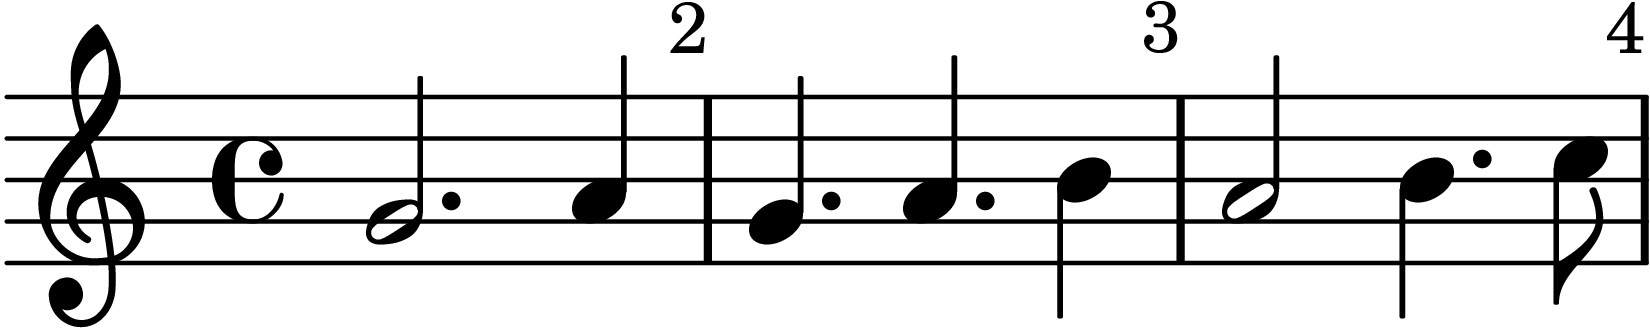
\includegraphics{fig/notes/point}
\end{center}

Теперь осталось прояснить вопрос, а как же быть с <<промежуточными>> нотами октавы, которые не имеют собственных имен, а обозначаются добавлением окончания <<-диез>> или <<бемоль>>. Дела в нотной записи обстоят примерно так же, как и с названиями, за тем лишь исключением, что знакомые уже нам значки \emph{альтерации}: диез ($\sharp$) и бемоль ($\flat$) добавляются \emph{перед} нотой. Все 12 нот малой октавы в восходящем порядке:
\begin{center}    
    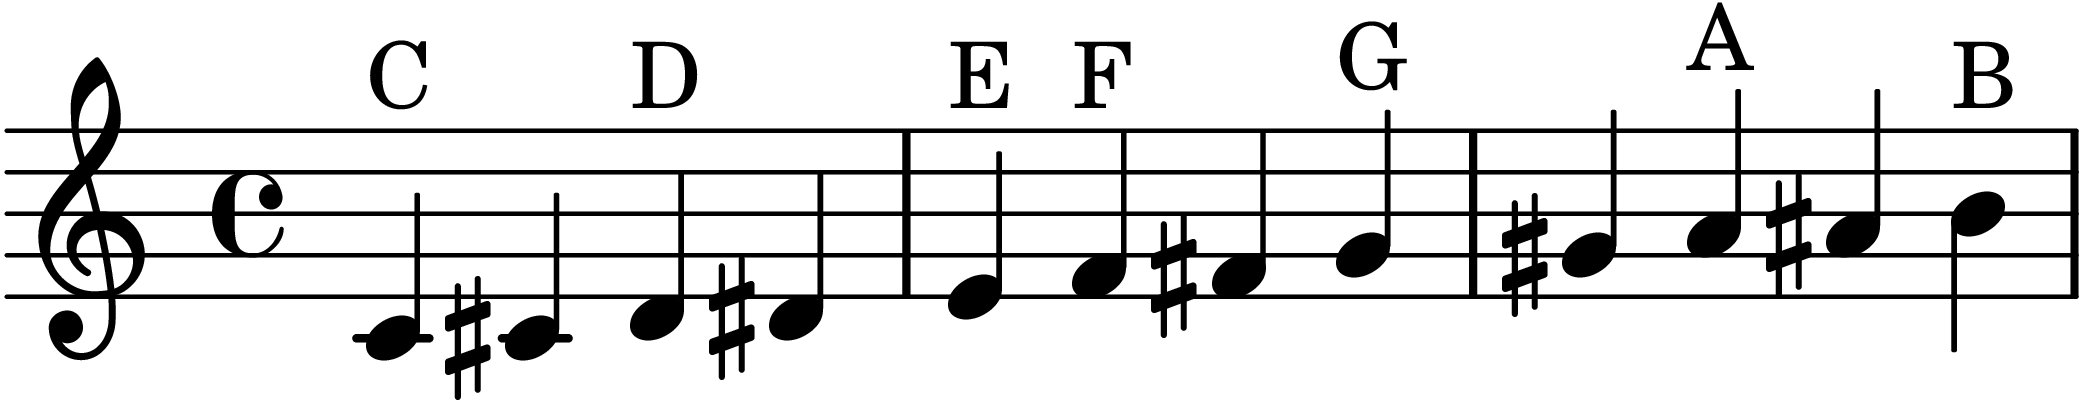
\includegraphics{fig/notes/octave-all-up}
\end{center}

В нисходящем:
\begin{center}    
    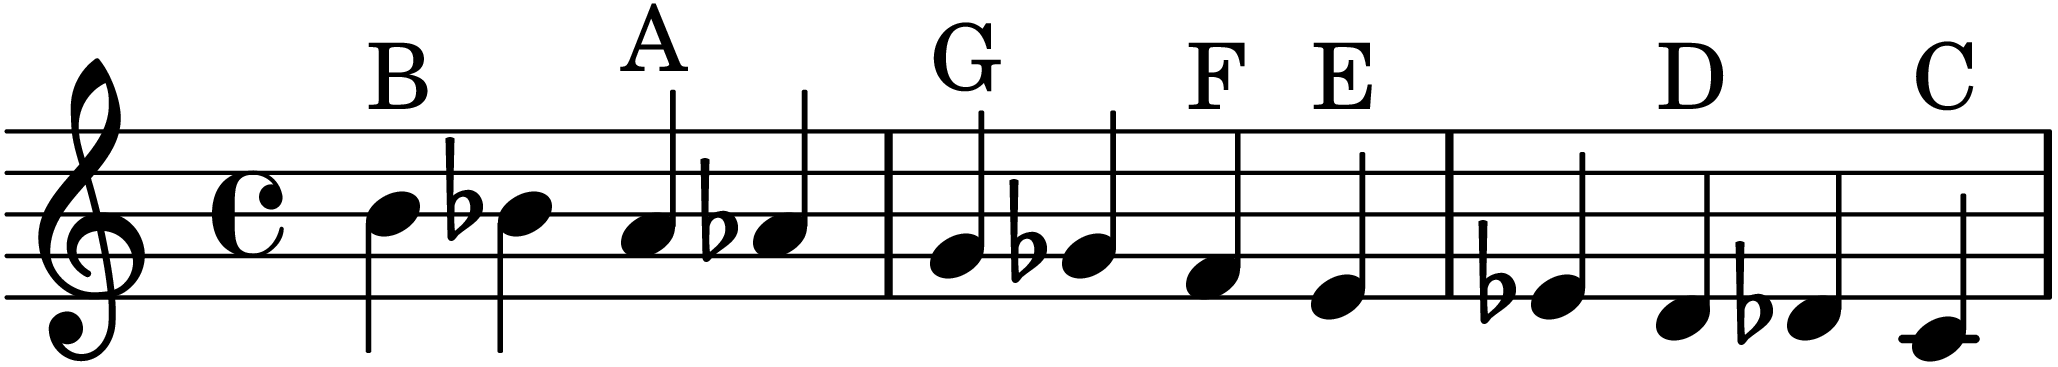
\includegraphics{fig/notes/octave-all-dn}
\end{center}

Как и положено, диез поднимает звук на полтона, а бемоль --- опускает. Кроме того, есть значки дубль-диез и дубль-бемоль, которые изменяют исходную ноту да целый тон. В данной записи в каждом такте звучит по две одинаковых четвертных ноты:
\begin{center}    
    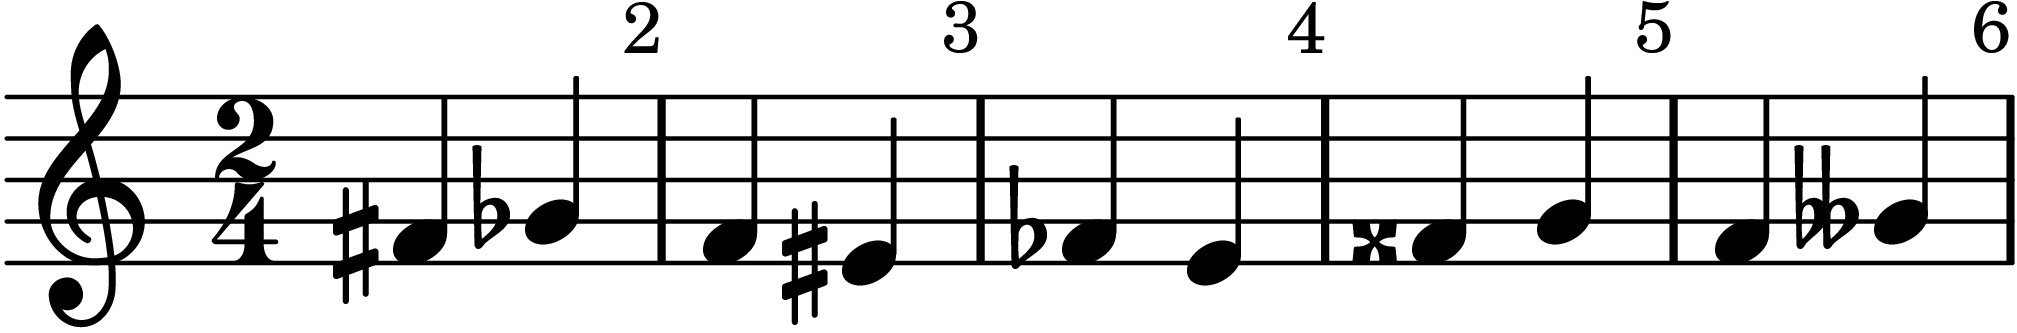
\includegraphics{fig/notes/sharp-flat}
\end{center}

\begin{itemize}
    \item В первом такте звучит две ноты ФА-диез (она же СОЛЬ-бемоль).
    \item Во втором такте: ФА, она же МИ-диез. Вы ведь помните, что между МИ и ФА расстояние в \emph{полутон}?
    \item В третьем: ФА-бемоль, она же МИ.
    \item В четвертом: ФА-дубль-диез, она же СОЛЬ.
    \item В пятом: ФА, она же СОЛЬ-дубль-бемоль.
\end{itemize}

В нотном письме есть особенность: знак альтерации, повышающий или понижающий ноту, действует до конца такта! Головоломка:
\begin{center}    
    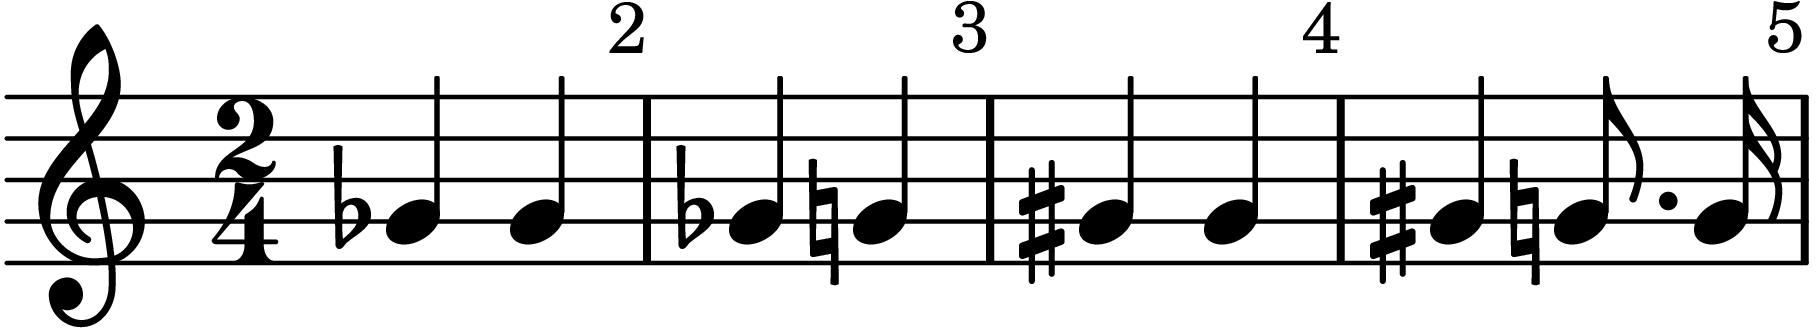
\includegraphics{fig/notes/bekar}
\end{center}
\begin{itemize}
    \item В первом такте звучат две ноты СОЛЬ-бемоль! Так как бемоль до конца такте понизил все нотки на второй снизу линии на полтона.
    
    \item А вот во втором такте звучит СОЛЬ-бемоль и СОЛЬ. Обратите внимание на значок, стоящий перед второй нотой --- он называется \emph{бекар}. Бекар отменяет действие знака альтерации и все последующие ноты на второй линии до конца такта будут просто СОЛЬ.
    
    \item Третий такт: две СОЛЬ-диез подряд.
    
    \item Четвертый: $\frac{1}{4}$ СОЛЬ-диез, $(\frac{1}{8} + \frac{1}{16}) = \frac{3}{16}$ СОЛЬ, $\frac{1}{16}$ СОЛЬ.
\end{itemize}

Знаки альтерации могут встретится не только перед нотой, а, например, сразу после ключа. В этом случае знак альтерации действует на все соотвествующие ноты (причём во всех октавах) до тех пор, пока не встретится очередной знак ключа. Встретившийся \emph{бекар} может отменить альтерацию только в течение такта. Очередная головоломка:
\begin{center}    
    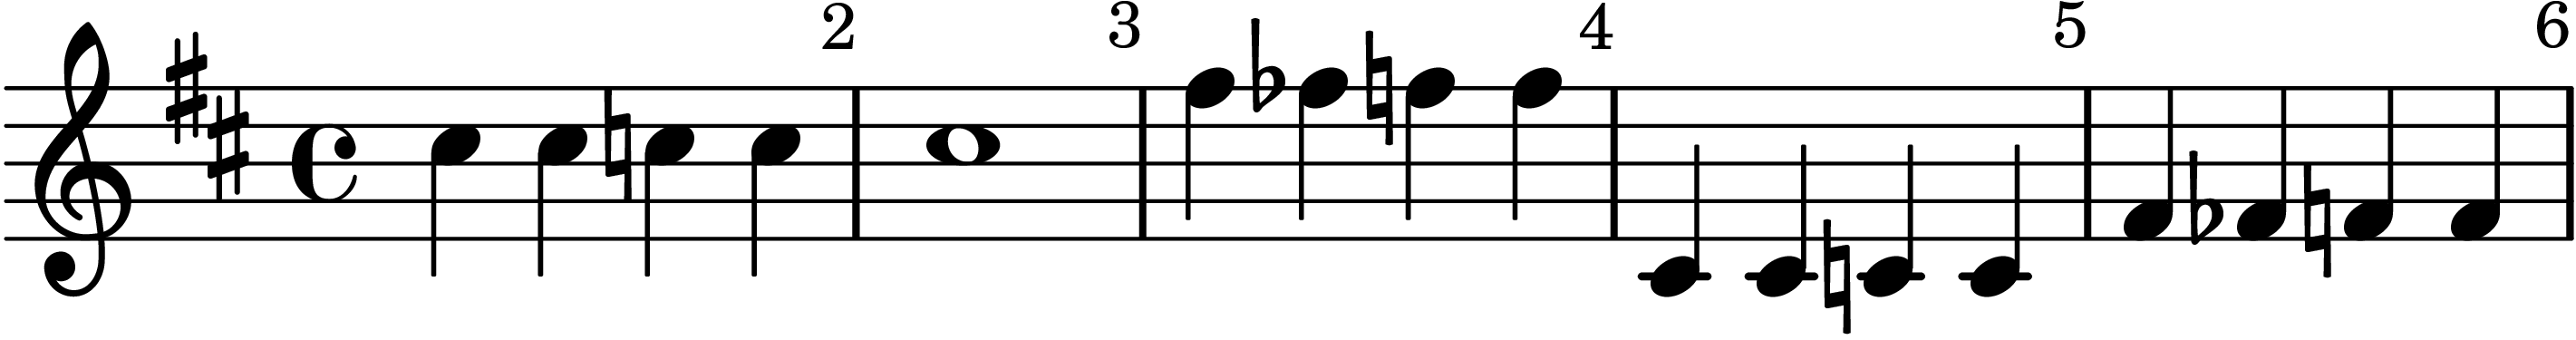
\includegraphics{fig/notes/tonality}
\end{center}

В приведенном примере будут автоматически повышены на полтона все ноты ФА (диез на пятой линии нотоносца) и все ноты ДО (диез в промежутке между третьей и четвертой линиями).
\begin{itemize}
    \item В первом такте две первые ноты --- ДО-диез. Затем бекар отменил действие диеза до конца такта, поэтому две последние ноты --- ДО.
    
    \item Во втором такте --- ДО-диез. Действует диез при ключе.
    
    \item В третьем такте первая нота --- ФА-диез. Затем действие диеза отменяет бемоль: вторая нота ФА-бемоль. Если бы следом не было бекара, то оставшиеся ноты были бы ФА-бемоль. Но бекар отменяет до конца такта все знаки альтерации, поэтому две последние ноты --- просто ФА.
    
    \item В четвертом такте две первые ноты --- ДО-диез. И хоть соответствующий диез после ключа стоял на линии ДО первой октавы, но действует он на ноты во \emph{всех} октавах. Так что все как в первом такте.
    
    \item В пятом такте все как в третьем, несмотря на разные октавы.
\end{itemize}

Читать ноты явно стало сложнее, потому что приходится держать в уме контекст: какие ноты понижаем, какие повышаем, а какие не меняем. Когда разберётесь с тем, что такое тональность (см. раздел \ref{ch:harmony:lad}) вы поймете, что такой подход имеет смысл с точки зрения экономии сил на рисование знаков альтерации, да и запись нот получаются более компактной и чистой.

Два одновременно сыгранных музыкальных звука называются \emph{интервалом}, а три и более --- \emph{аккордом}. В этом случае ноты просто пишутся друг над другом. Аккорд <<ДОМИСОЛЬка>> в разных длительностях:
\begin{center}
    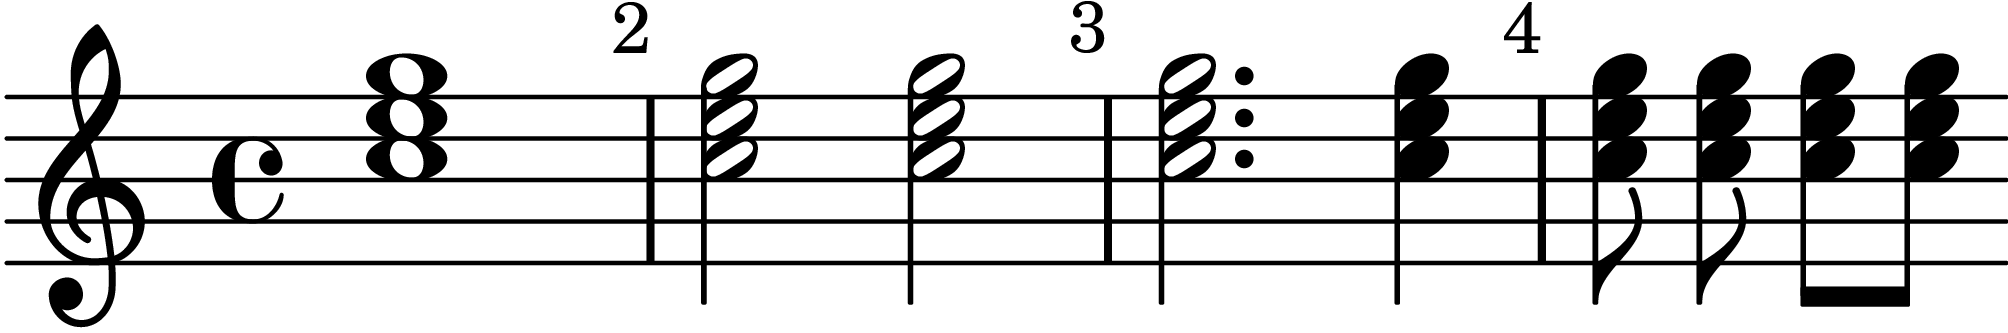
\includegraphics{fig/notes/chord}
\end{center}

Теперь настало время поговорить о самом важном элементе музыки: тишине. Внимание: \emph{пауза}. Паузу держат в тех же долях условной единицы длительности, что и ноты, только вот лиговать паузы не надо: тишина и есть тишина. Заполним такты тишиной и музыкой (посчитайте совместные длительности пауз и нот, должно получиться $\frac{4}{4}$): 
\begin{center}
    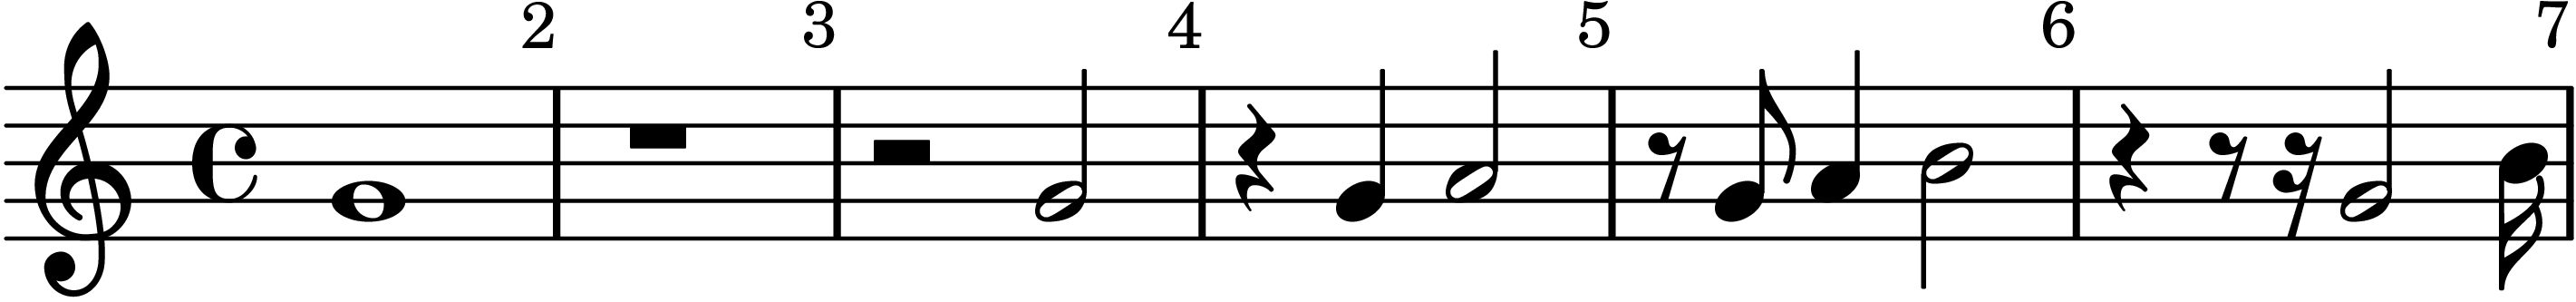
\includegraphics{fig/notes/pause}
\end{center}
\begin{itemize}
    \item В первом такте пауз нет: весь такт звучит СОЛЬ.
    \item Весь второй такт молчит \emph{целая} пауза, длительность которой --- целая условная единица. Толстая чёрточка точно под четвертой снизу линией нотоносца.
    \item В начале третьего такта --- \emph{половинная} пауза. Та же чёрточка, но над третьей линией.
    \item Четвертый такт начинается с четвертной паузы. Словами сей крючок не описать.
    \item Пятый такт начинается с паузы, длящейся восьмую часть условной единицы. Характерная косая черточка с засечкой (флажком).
    \item Шестой такт начинается с паузы в $\frac{7}{16}$ долей условной единицы. Эта пауза состоит из четвертной, восьмой и шестнадцатой пауз: $\frac{1}{4} + \frac{1}{8} + \frac{1}{6} = \frac{7}{16}$. Шестнадцатая пауза выглядит как восьмая, только добавилась еще одна засечка. 
\end{itemize}

В изображении пауз дела обстоят как и с нотами: начиная с <<восьмых>> --- только засечки (флажки) добавляются. Добавился флажок --- длительность уменьшилась вдвое. Мы не рассматривали ни ноты, ни паузы длительностью короче шестнадцатых, но надо сказать, что в природе они есть. Теоретически можно делить условную единицу на два хоть до бесконечности, но какой робот сыграет такую музыку?

Напоследок пару слов о темпе. То есть о том, какой интервал времени соответствует этой самой дробящейся условной единице длительности? Как его задать? Композиторы прошлого использовали довольно сложную систему названий, определяющих скорость исполнения: largo (очень медленно), adagio (медленно), andante (умеренно), allegro (весело), presto (быстро). А уж вариаций вроде allegretto moderato (умеренно оживленно) было не счесть\ldots Доходило до драк, ибо <<аллегретто модерато>> для каждого свое. 

Сейчас обычно делают так: задают длительность четвертной ноты в долях минуты и, чтобы старички не волновались, пишут, мол <<аллегретто>> и чутка даже <<модерато>>. Главное без ошибок:
\begin{center}
    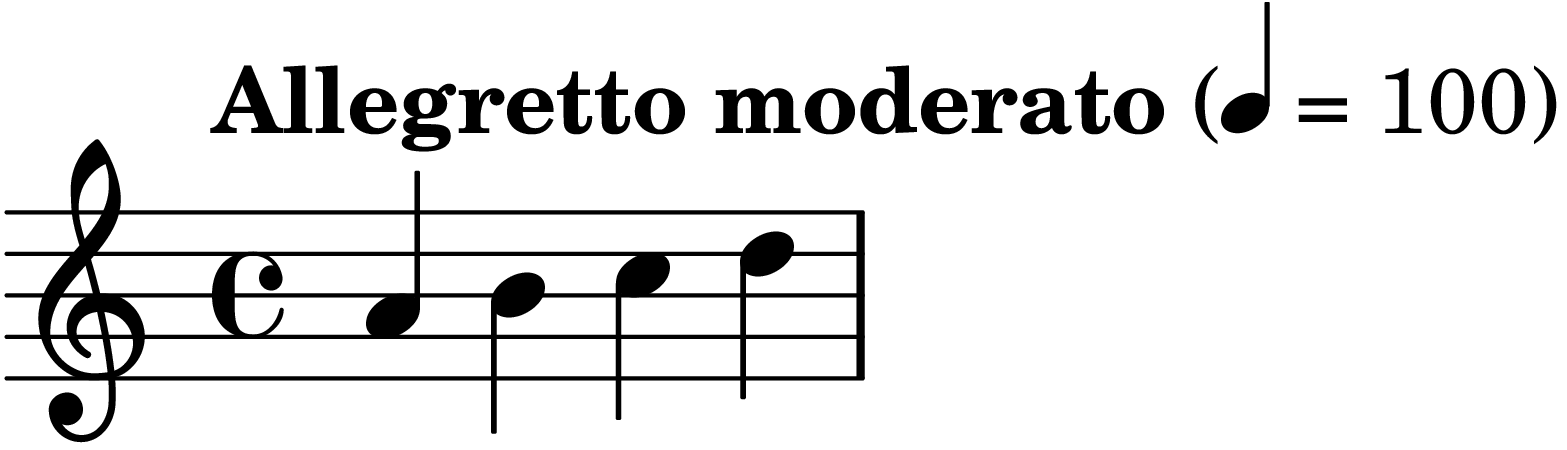
\includegraphics{fig/notes/tempo}
\end{center}

Здесь (в скобочках, после <<аллегретто модерато>>) объявлено, что за минуту нужно успеть сыграть ровно 100 четвертных нот (а стало быть 50 половинных, 25 целых, 200 восьмых и т.д.). На любом испарвном метрономе выставляется темп в 100 щелчков в минуту и музыкант тренируется <<под метроном>>. И нет поводов для мордобоя. 

Мы не будем досконально разбираться во всех тонкостях нотной записи, коих немало. Мы уже рассмотрели достаточный минимум, который при необходимости поможет разобраться в более сложных темах. В качестве доступных справочных пособий, в которых нотная грамота представлена во всем её многообразии, можно рекомендовать книги \cite{bib:alekseev:MusicTheory,bib:vahromeev:Theory}.

Также стоит сказать, что гитара, несмотря на свою простоту и скромный диапазон, как музыкальный инструмент имеет выразительные возможности, недоступные многих другим инструментам: на гитаре можно играть флажолеты, подтяжки, вибрато, мертыве (как бы страшно не звучало) ноты, барабанить (научно --- перкуссия) и много, много чего ещё. И всё это выражается в особых, специфичных для гитары, пометках на нотах.

Если вы возьмёте нотную тетрадь и попробуете переписать, например несколько учебных пьес или этюдов (что, кстати, крайне полезно сделать!), то заметите, что шариковой ручкой писать ноты не совсем удобно (особенно штриховать овальчики четвертных и более коротких нот). Нотная грамота создавалась во времена перьевых ручек, а точнее даже очиненных перьев, а для такого пишущего инструмента провести линии разной толщины --- дело плёвое. Каллиграфии в те времена учили всех, и наши предки писали очень красивые ноты гораздо быстрее нас --- инструменты и навыки позволяли.

Тем кто захочет издать свою музыку в высоком качестве, можно рекомендовать \cite{url:lilypond} --- свободную программу lilypond\footnote{Я шучу, использовать lilypond, если вы не программист (не гик, не математик, не фанат \LaTeX,\ldots) и с английским (или с чешским, немецким, испанским, французким, в общем практически с любым языком, увы, за исключением Русского) напряженно, то не стоит ломать себе психику. В противном случае дерзайте: изучение lilypond-нотации позволит глубже понять музыку. В документации к lilypond вы также найдёте определения многих музыкальных терминов, а многочисленые примеры и, например, программа friscobaldi позволят вам учиться нотной грамоте в интерактивном режиме} и всё, что создано на её основе.


\section{Как это сыграть на гитаре? Гитарная табулатура}

Мало понять, какие музыкальные звуки скрываются за нотами, надо еще суметь <<доcтать>> их из гитары. Устройство гитары мы обсуждаем в разделе \ref{ch:guitar}, но и так понятно, что основной вопрос на начальном этапе: <<На каком ладу зажать струну, чтобы прозвучала нужная нота?>>. 

Ответ на этот вопрос дает \emph{табулатура} --- способ записи музыки, отражающий особенности инструмента. В простонародье табулатуру называют: <<табы>>.

В гитарном случае табулатура выглядит примерно так:
\begin{center}
    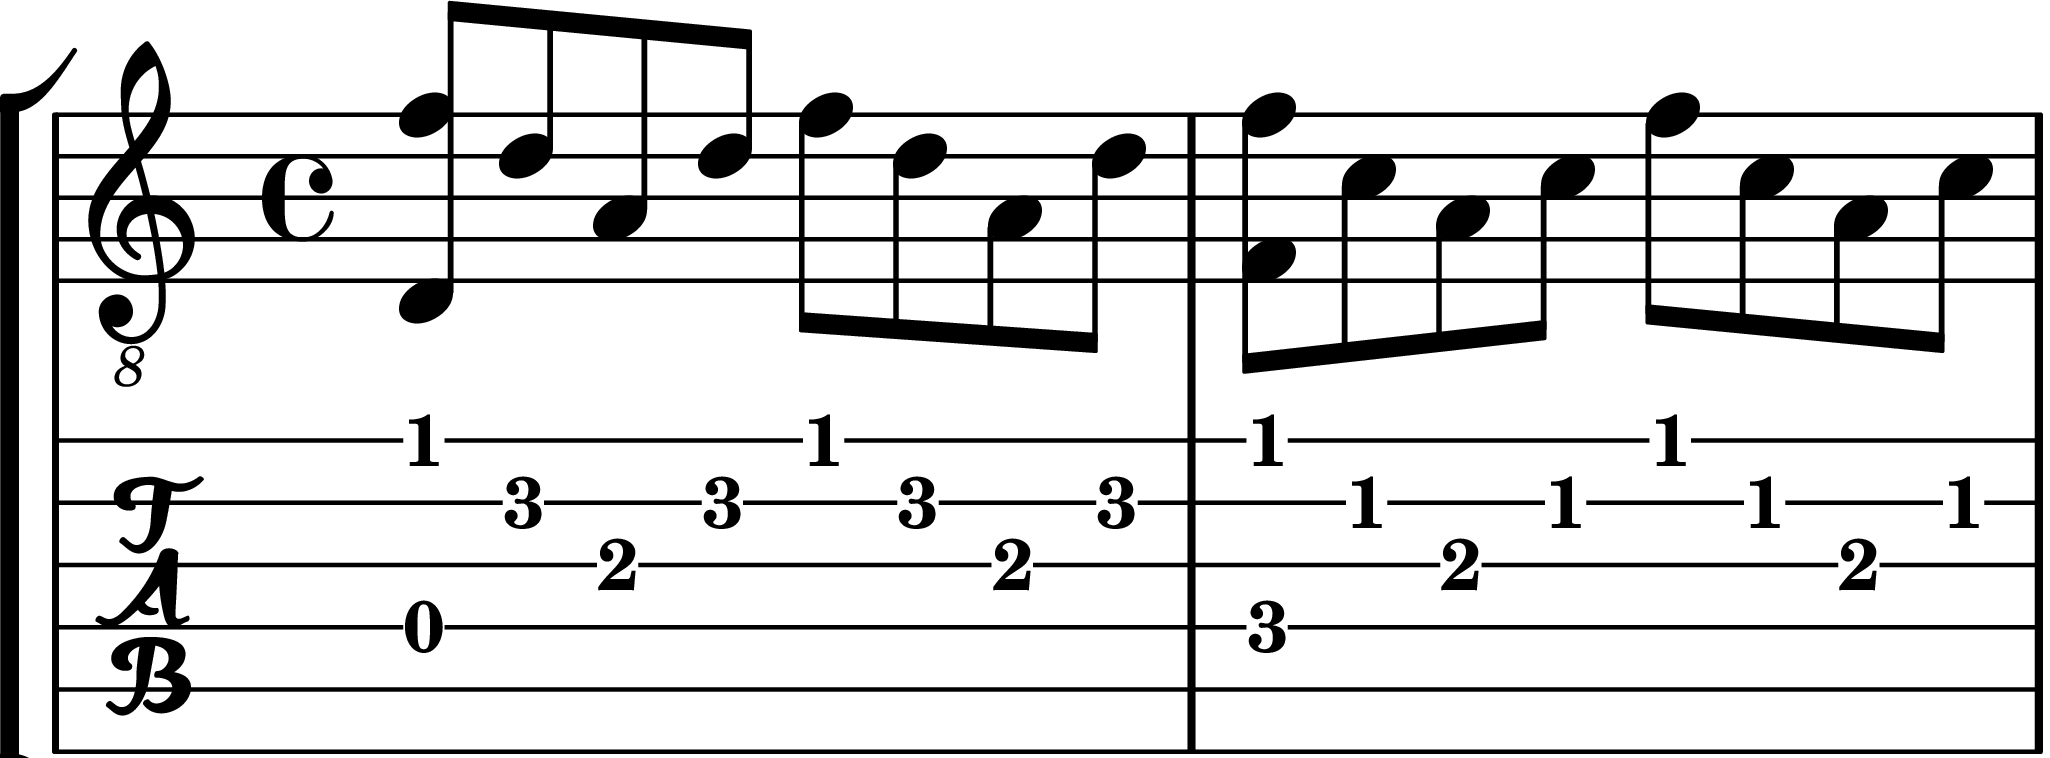
\includegraphics{fig/notes/tab}
\end{center}

Под линейкой нотоносца размещается шесть линий (подписанных словом <<TAB>>), соотвествующих гитарным струнам --- это и есть табулатура. Верхняя линия соотвествует первой струне на гитере, а нижняя, соответственно, шестой, басовой струне. Непосредственно под нотами на линии табулатуры пишется номер лада, на котором нужно зажать и сыграть соотвествующую этой линии струну.

Немного разберем приведенную запись. Итак, вначале мы играем две ноты одновременно: ФА первой октавы (1-й лад на первой струне) и РЕ малой октавы (зажатая на нулевом ладу, т.е. открытая четвертая струна). Потом РЕ первой октавы (третий лад второй струны). И т.д.

Приведенная в качестве примера табулатура без нотоносца над ней бессмысленна, так как без нот потеряется информация о длительности извлекаемых звуков. Но все чаще в Интернет можно увидеть табулатуры для новичков, в которых отсутствует нотоносец, но у номеров ладов появляютя характерные нотные <<хвостики>>, опредедяющие длительность.

Табулатуры является существенным подспорьем для новичка. Но, набравшись опыта, гитарист не будет в них нуждаться, потому что без подсказок будет знать где на грифе находится нужная нота.
